\documentclass[fleqn,10pt]{wlscirep}\usepackage{knitr}
\usepackage[utf8]{inputenc}
\usepackage[T1]{fontenc}
\usepackage{graphicx}
\usepackage{tcolorbox}
\usepackage{amsmath}
%\usepackage[backend=biber]{biblatex}
%\addbibresource{sample.bib, R-Pckgs.bib}
%\bibliography{sample, R-Pckgs}



% New Commands
\makeatletter
\newcommand{\distas}[1]{\mathbin{\overset{#1}{\kern\z@\sim}}}%
\newsavebox{\mybox}\newsavebox{\mysim}
\newcommand{\distras}[1]{%
    \savebox{\mybox}{\hbox{\kern3pt$\scriptstyle#1$\kern3pt}}%
    \savebox{\mysim}{\hbox{$\sim$}}%
    \mathbin{\overset{#1}{\kern\z@\resizebox{\wd\mybox}{\ht\mysim}{$\sim$}}}%
}
\makeatother


% title

\title{Development and testing of a nearest neighbors clinical prediction model for physical function after total knee arthroplasty}

\author[1,*]{Andrew Kittelson}
\author[1]{Tim Loar}
\author[2,3,+]{Chong H. Kim}
\author[2,+]{Kathryn Colborn}
\author[4,+]{Stef van Buuren}
\affil[1]{Department of Physical Medicine \& Rehabilitation, University of Colorado Physical Therapy Program, Aurora, USA}
\affil[2]{Department of Biostatistics \& Informatics, University of Colorado, Aurora, USA}
\affil[3]{Department of Clinical Pharmacy, University of Colorado, Aurora, USA}
\affil[4]{Department of Methodology \& Statistics, University of Utrecht, Utrecht, The Netherlands}

\affil[*]{andrew.kittleson@ucdenver.edu}

\affil[+]{these authors contributed equally to this work}

%\keywords{Total Knee Arthroscopy, Prediction model, Personalized reference chart}

\begin{abstract}
Example Abstract. Abstract must not include subheadings or citations. 
\end{abstract}


%--------------------------------------------------------------------
% PATH setup
%--------------------------------------------------------------------
\graphicspath{{../figure/}{./figure/}}


%--------------------------------------------------------------------
% knitr setup
%--------------------------------------------------------------------


\IfFileExists{upquote.sty}{\usepackage{upquote}}{}
\begin{document}

\flushbottom
\maketitle
% * <john.hammersley@gmail.com> 2015-02-09T12:07:31.197Z:
%
%  Click the title above to edit the author information and abstract
%
\thispagestyle{empty}

%\noindent Please note: Abbreviations should be introduced at the first mention in the main text – no abbreviations lists. Suggested structure of main text (not enforced) is provided below.


%--------------------------------------------------------------------
% Introduction
%--------------------------------------------------------------------

\section*{Introduction}

Total Knee Arthroplasty (TKA) is the most commonly performed inpatient elective surgery in the United States, at approximately $700,000$ procedures per year\cite{bernstein2014dramatic}. Although TKA is regarded as effective, the clinical course is highly variable. Depending on the patient, recovery of physical function can occur rapidly (within weeks), or it can be an arduous, months$-$long process\cite{bade2010outcomes,judd2012muscle}. Moreover, the surgical population is remarkably heterogeneous—some patients engage in sporting activities (e.g., tennis, skiing)\cite{weiss2002functional}, while others struggle to ambulate at walking speeds sufficient for independence in the community. There is no such thing as the ``average'' patient.

To achieve the ideals of person-centered care, and also because TKA is an elective procedure, clinical decisions should be anchored to the individual patient. Yet the determination of an individual patient’s functional prognosis is challenging.  Prediction models have been developed in TKA, but these models have several limitations: 1) they perform poorly in out$-$of$-$sample testing\cite{sanchez2018development}, 2) they are based on mathematical functions that are unlikely to be flexible enough to realistically portray the clinical course across all patients\cite{kennedy2008assessing}, or 3) they predict functional outcomes at discrete postoperative time points, which may not overlap with the time frame during which patients are undergoing postoperative care and clinical monitoring\cite{mizner2005preoperative}. 

Neighbors-based predictions—where an index patient’s prognosis is estimated from the observed recovery data of previous similar patients (i.e., the patient’s ``neighbors”)—addresses many of these limitations.  The parameters of the prediction (and the shape of the prognostic trajectory) are allowed to vary substantially across individuals. This may in fact be necessary to accommodate the heterogeneity in recovery following TKA\cite{page2015distinguishing}. Additionally, for any individual patient, the prognosis is estimated from a subset of patients with similar characteristics. This may improve the generalizability of the predictions over commonly used mathematical approaches (e.g. multiple regression, mixed effects models), where the parameters of a prediction model are heavily influenced by the characteristics of the sample in which it is developed, potentially limiting its application in samples with different characteristics (e.g. different sociodemographic profile of patients, etc.). 

The purpose of this study was to develop a clinical prediction model for functional recovery after TKA surgery, using a novel neighbors-based prediction approach\cite{van2014curve}. The outcome of interest for this study was the Timed Up and Go (TUG) test, a clinically feasible test of mobility and a surrogate of lower extremity strength. We utilized a combination of clinical and research data, collected longitudinally over the first six months following surgery. We divided the patients temporally (by date of surgery) into a training set and test set. The training set was used to refine the procedures and to supply the seed data for generating nearest neighbors' predictions. The performance of this approach was then adjudicated against data from the test set as a preliminary validation. 

%--------------------------------------------------------------------
% Results
%--------------------------------------------------------------------

\section*{Results}
\subsection*{Descriptive statistics}

\begin{figure}[!htbp]
\centering
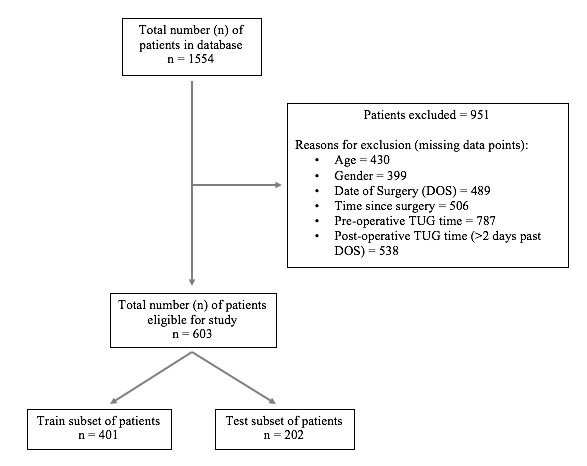
\includegraphics[width=\linewidth]{fig1}
\caption{Study population enrollment flowchart}
\label{fig:fig1}
\end{figure}



In the training data set we analyzed information on 397 patients with 1,339 post-operative TUG observations. We used information information on 201 patient (604 observations) in the testing data. Patient characteristics from training and testing data are shown in Table \ref{tab:tab1}. Broadly, the ratio of male and BMI were similar across the two data sets while there were statistically significant difference in age and baseline TUG time. Compared to the patients in the training data, patients were approximately 2 years older and had a 1 second faster baseline TUG times on average. 

\begin{table}

\caption{\label{tab:tab1}Baseline Characteristics of Training and Testing Set}
\centering
\resizebox{\linewidth}{!}{
\begin{tabular}[t]{lccr}
\toprule
  & Train & Test & p^a\\ & (N = 398, \# TUG Obs = 1340) & (N = 201, \# TUG Obs = 604) &  \\
\midrule

Age (years) (mean (sd)) & 64.04 (8.43) & 65.90 (8.84) & 0.012\\
Gender = Male (\%) & 185 (46.6) & 84 (41.6) & 0.280\\
BMI (kg/m\textasciicircum{}2) (mean (sd)) & 31.33 (5.82) & 31.98 (6.20) & 0.208\\
Baseline TUG (sec) (mean (sd)) & 9.98 (4.95) & 11.00 (5.04) & 0.018\\
\bottomrule
\multicolumn{4}{l}{\textsuperscript{a} Continuous variables tested with one-way analysis of variance; Categorical variables tested with}\\
\multicolumn{4}{l}{$\chi^2$ test}\\
\end{tabular}}
\end{table}




\subsection*{Nearest Neighbors Selection and Model Tuning}




\subsubsection*{Matching characteristics}

Based on the stepwise AIC method, age ($\beta = $ 3.67e-02; $\text{p} = $ 1.26e-03), gender ($\beta = $ 9.19e-01; $\text{p} = $ 1.22e-06), BMI ($\beta = $ 3.72e-02; $\text{p} = $ 2.27e-02), and preoperative TUG time ($\beta = $ 2.05e-01; $\text{p} = $ 1.82e-22) were selected as having statistically significant effect on 90-day post-operative TUG time. Preoperative TUG time was the most important matching characteristic, a change in 1 standard deviation of preoperative TUG had 4.67 times the impact on 90-day post-operative TUG time, compared to a 1 standard deviation change in BMI.

\subsubsection*{Number of Matches}



The optimal number of matches selected was $n = $ 35 based on the lowest weighted bias (5.29e-03), coverage (5.04e-01), and precision (2.33e+00) score (Figure \ref{fig:fig_BCCGo_loocv}). 

\begin{figure}[!htbp]
\centering
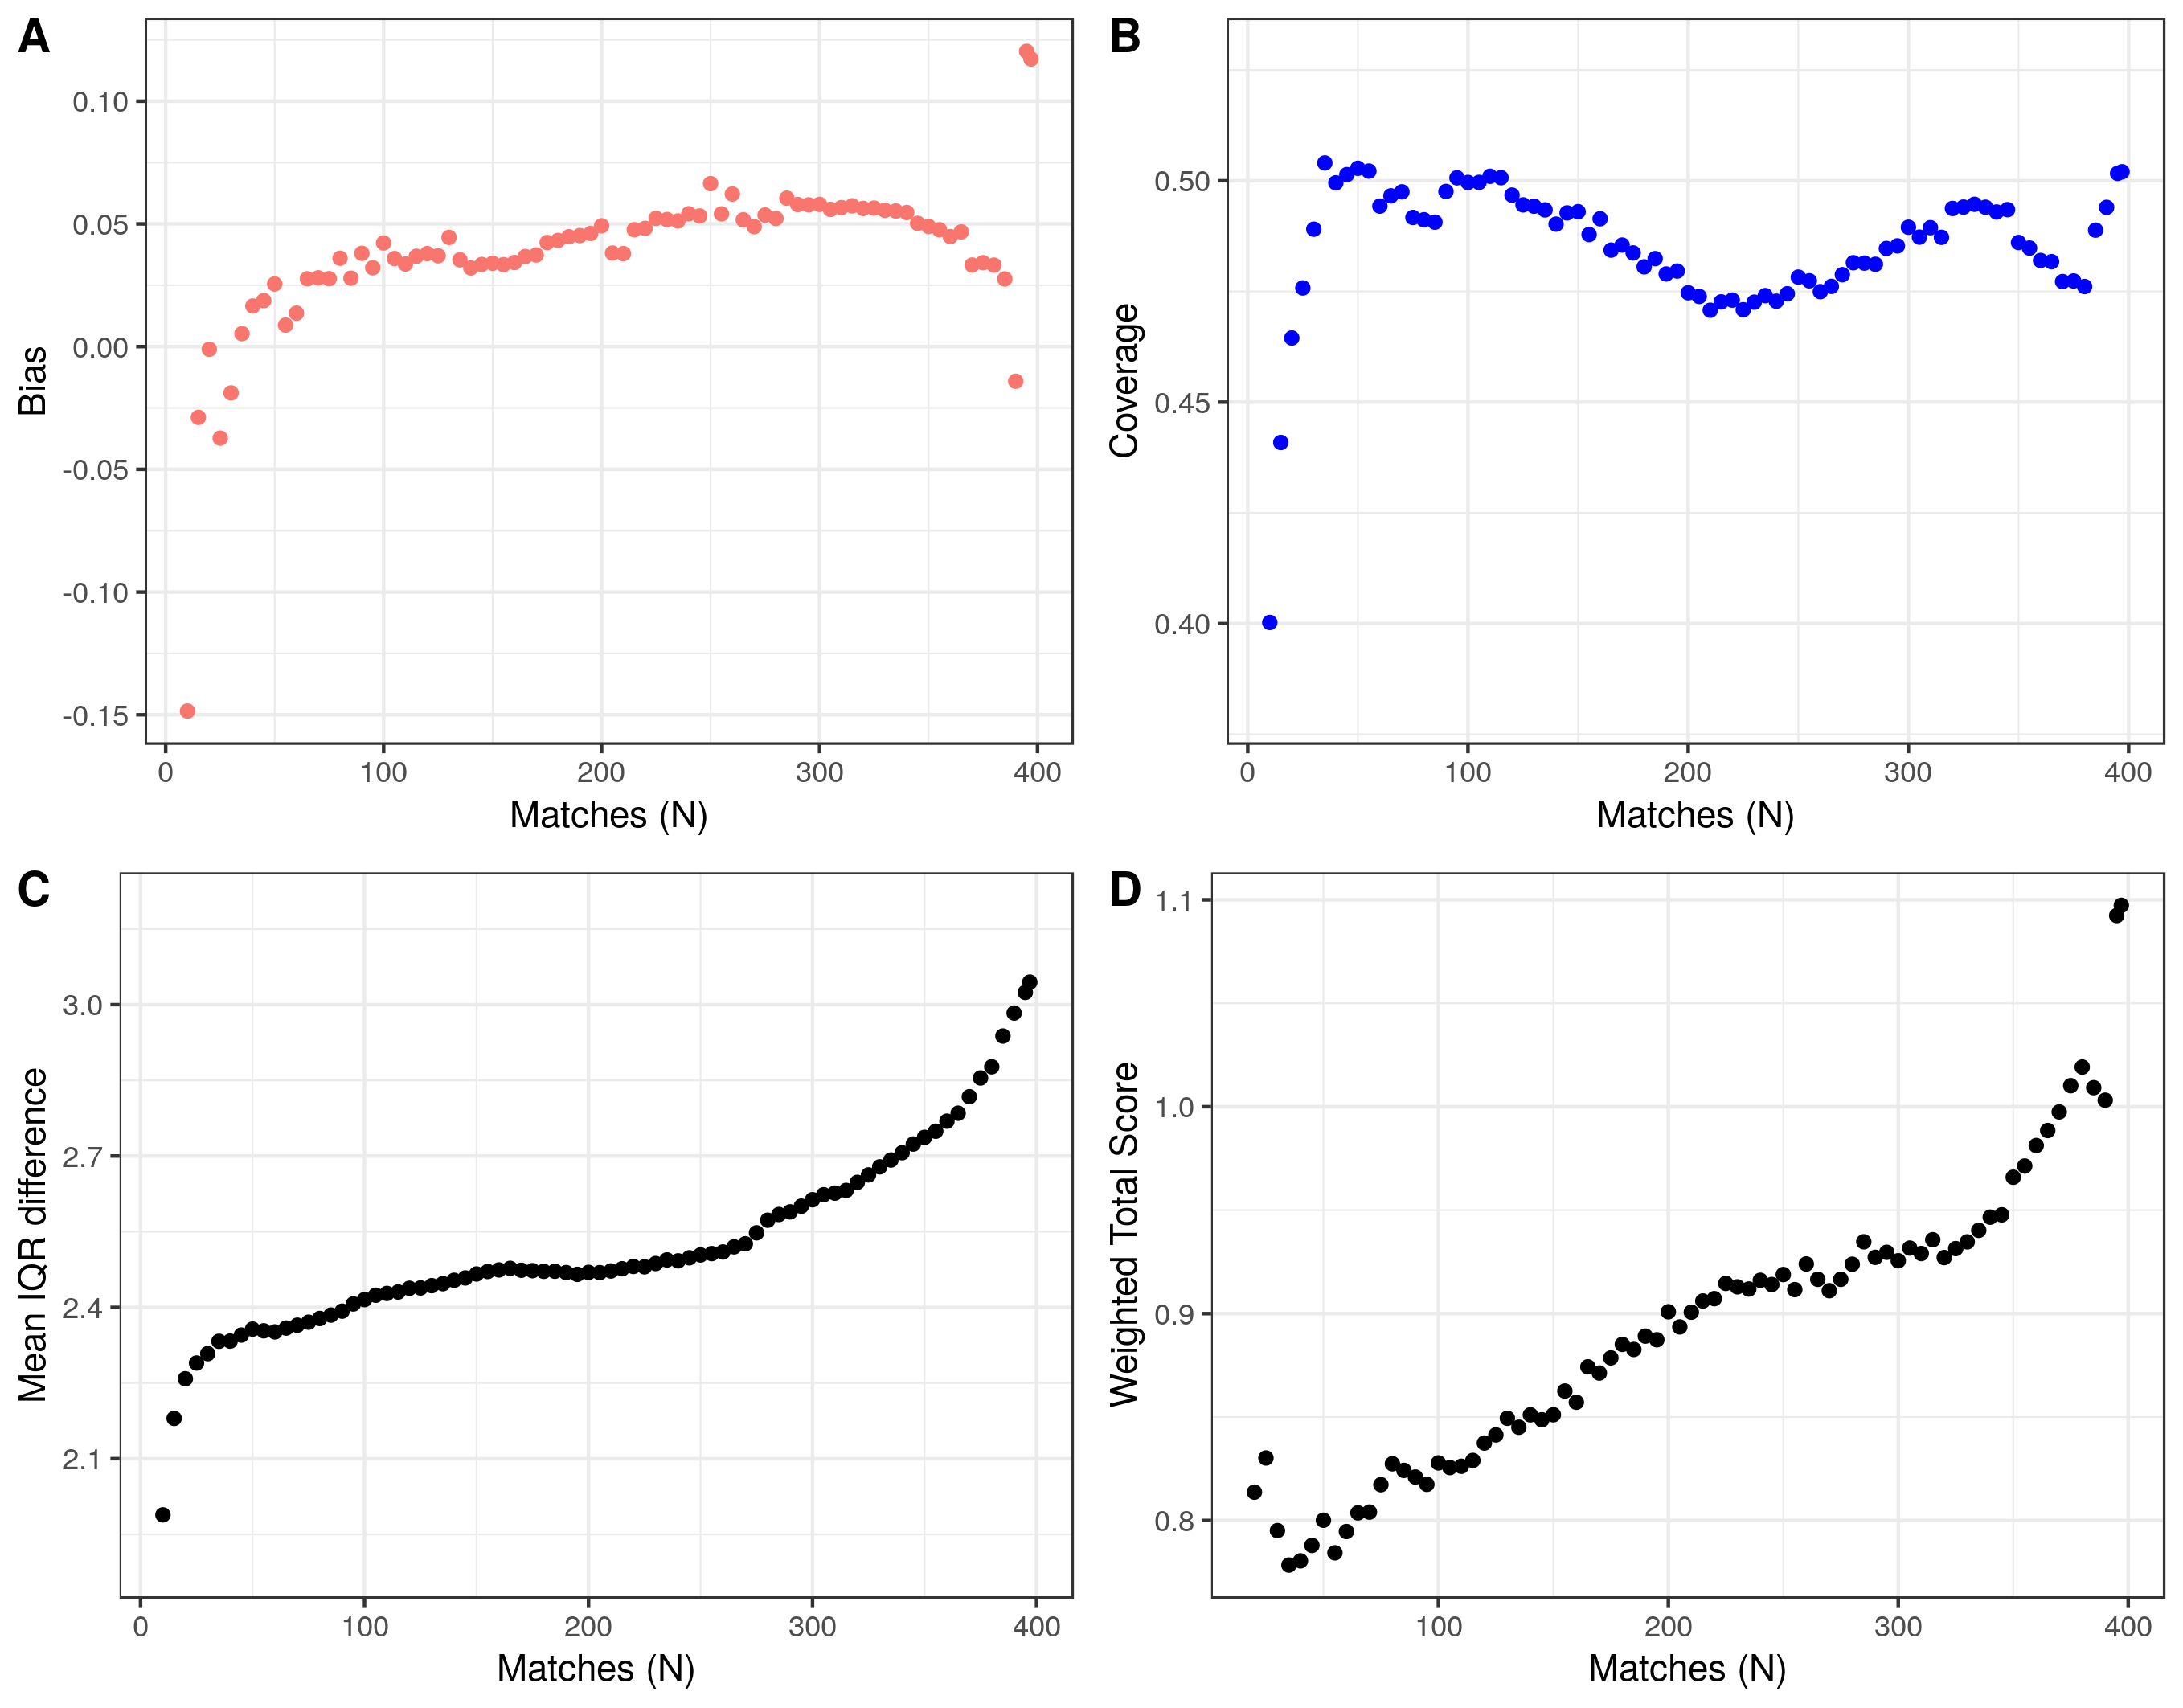
\includegraphics[width=\linewidth]{fig_BCCGo_loocv}
\caption{Bias, coverage, and precision plot using Box-Cox-Cole-Green distribution for location, shape, and scale for gamlss}
\label{fig:fig_BCCGo_loocv}
\end{figure}


\begin{figure}[!htbp]
\centering
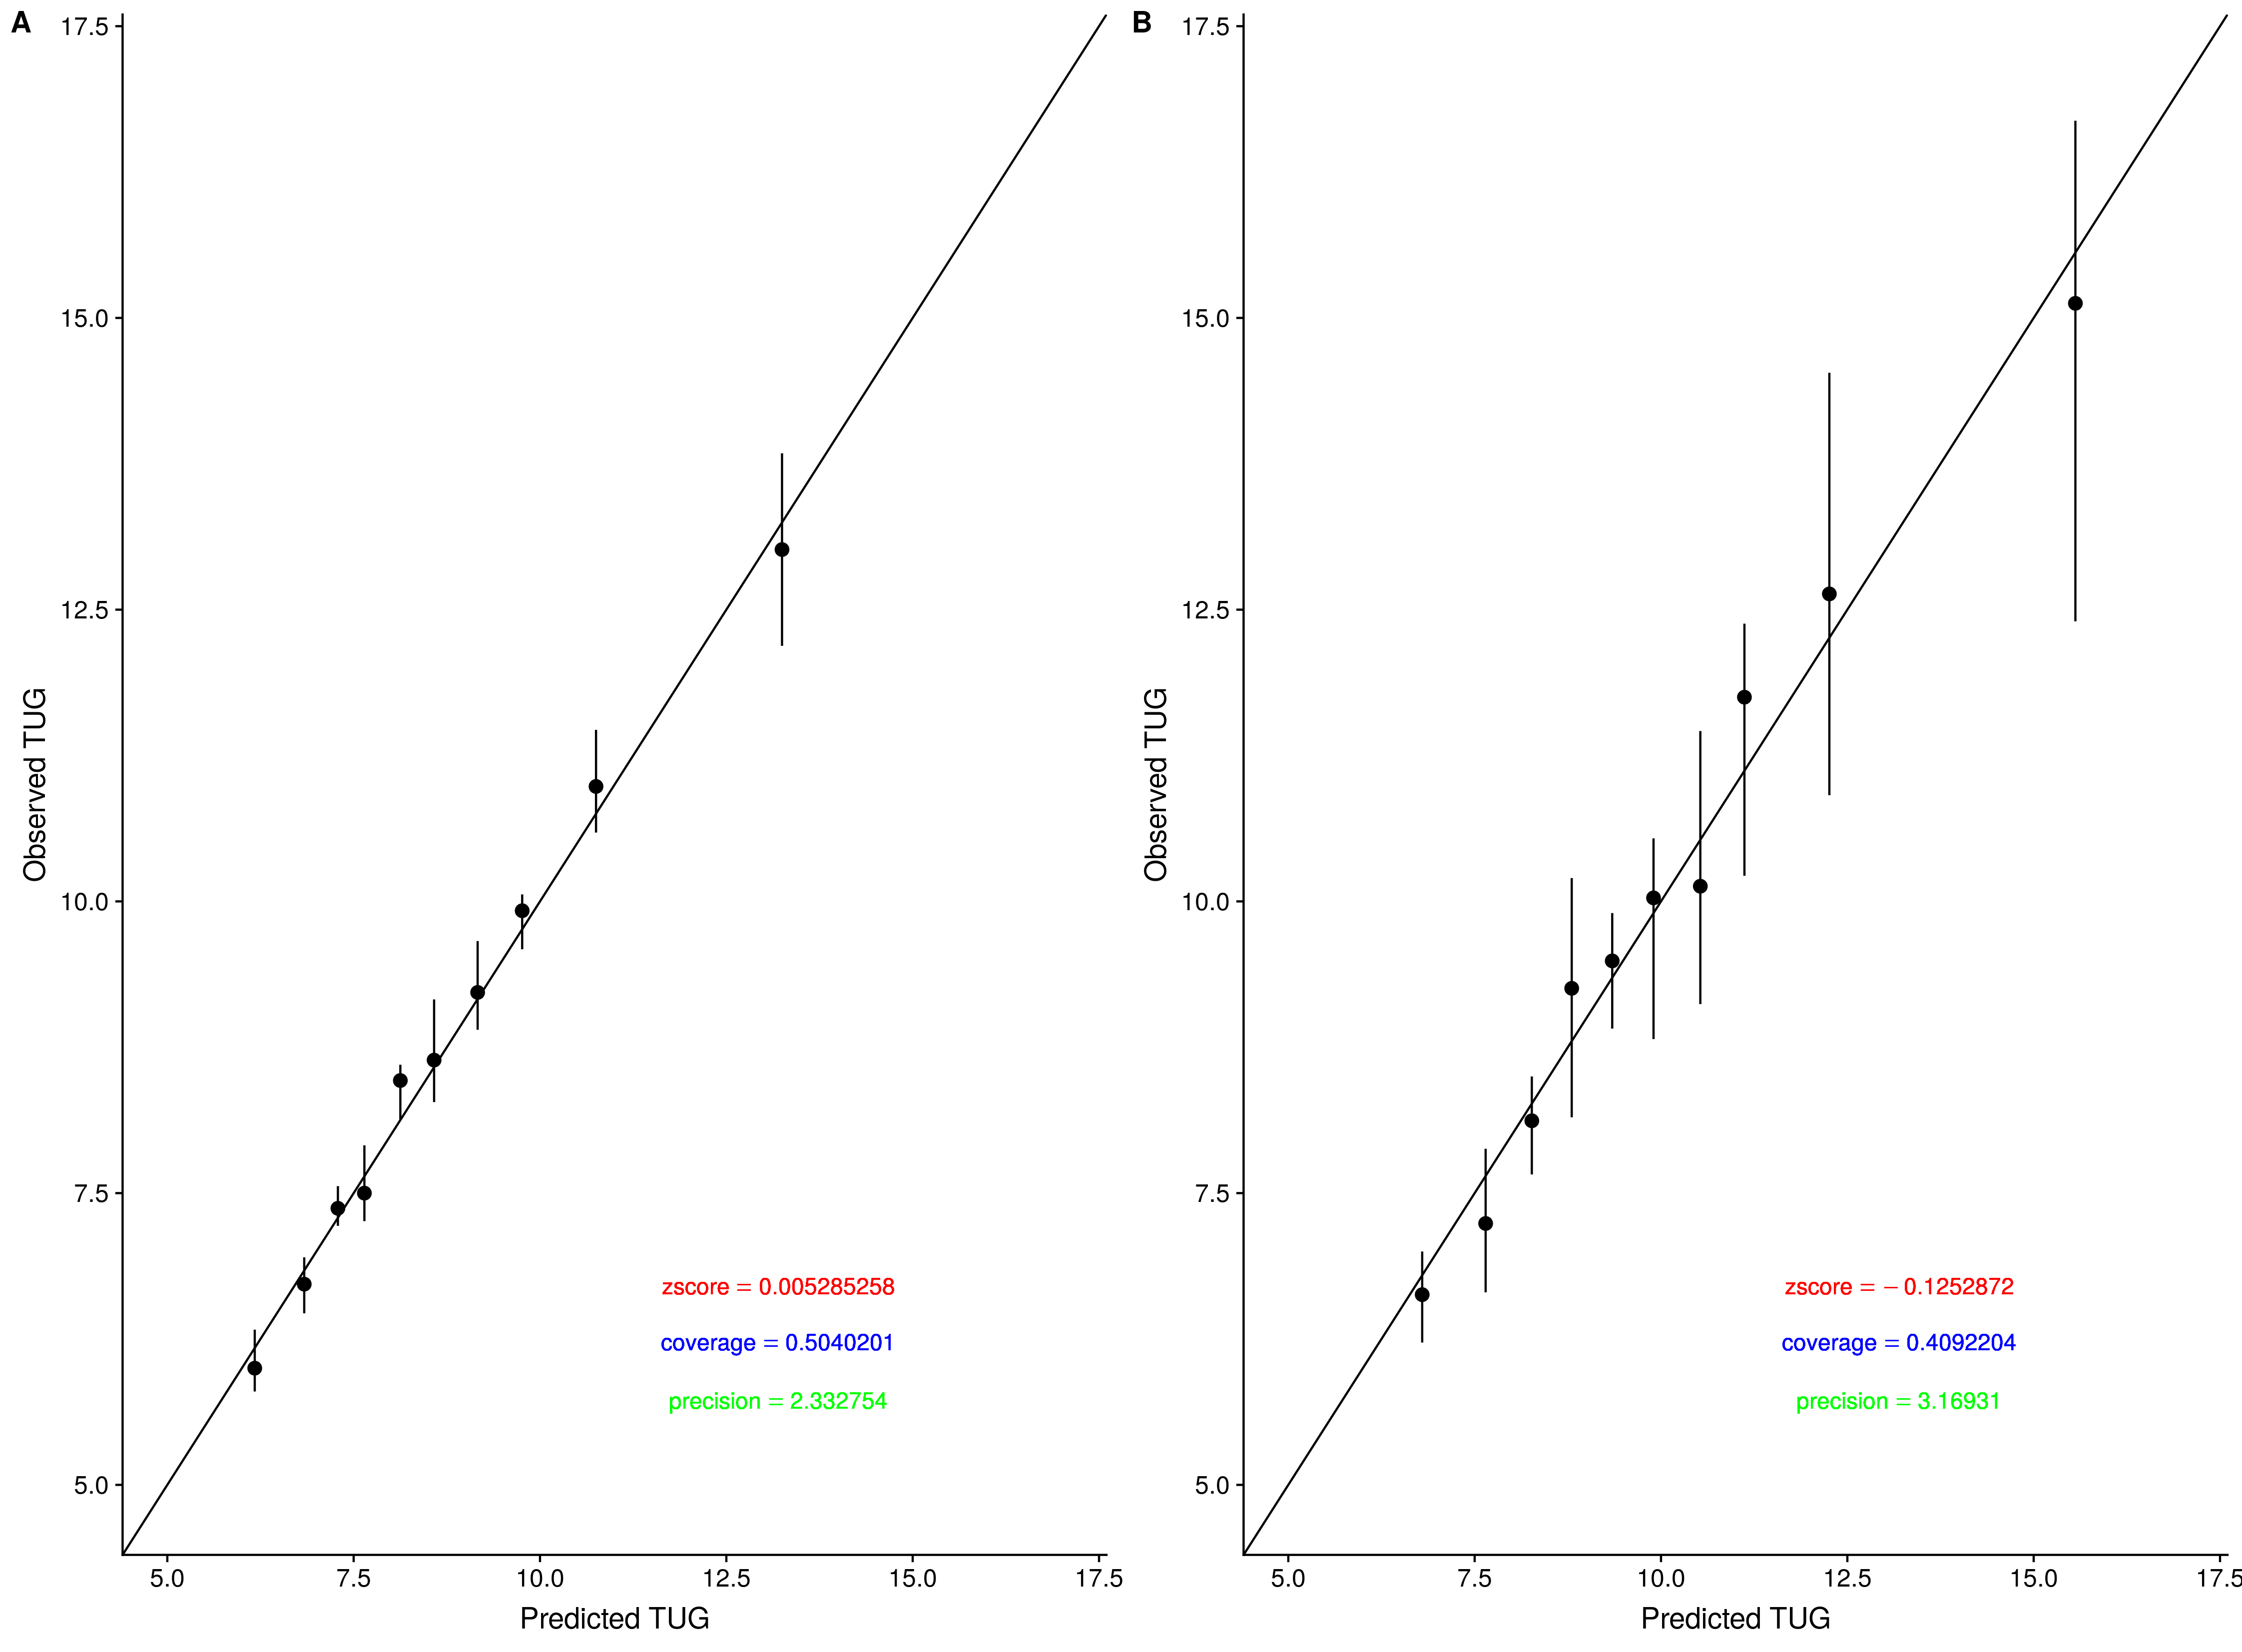
\includegraphics[width=\linewidth]{fig_BCCGo_cal}
\caption{Bias, Coverage, and precision plot using Box-Cox-Cole-Green distribution for location, shape, and scale for gamlss}
\label{fig:fig_BCCGop_cal}
\end{figure}

\subsubsection*{Performance via Internal and External Validation}

The average bias, coverage, precision, and the weighted score for all TUG predictions in the training data was 0.0052853, 0.5040201, 2.3327538, and 0.7784423, respectively (Figure ~\ref{fig:fig_BCCGo_loocv}). Model calibration was good, with close agreement between predicted and observed values of post-operative TUG times (Figure ~\ref{fig:fig_BCCGop_cal}). 


\section*{Discussion}

We developed and tested a novel, neighbors-based prediction for physical function following TKA. Body Mass Index (BMI), sex, age, and preoperative TUG time were used to identify the 35 nearest neighbors to an index patient, via predictive mean matching.  The observed data from these neighbors were then used to develop an estimate of an index patient’s TUG prognosis. By within-sample testing, predictions performed well, with very low bias ($<0.01$ standard deviations, on average) and accurate coverage (proportion of realized observations within the IQR $= 0.508$). On average, the 50\% prediction window was 2.29 seconds, which is within the measurement error of the TUG test in this population. The interpretation of this result is as follows: with greater than 50\% confidence (on average), we were able to predict patients’ TUG scores across all postoperative time points within the measurement error of the test. Compared to a population-level estimate, this amounts to a 24\% improvement in precision. 

In a temporally distinct test sample (more recent surgical dates) the predictions performed accurately across all deciles of observed data (Figure \ref{fig:fig_BCCGop_cal}). This was especially encouraging given the differences in patient characteristics between training and test datasets (Table \ref{tab:tab1}) and considering national-level changes to TKA care, which occurred during the period of data collection (cite CJR). To our knowledge, this is the first study to successfully externally validate a prediction model for physical function in TKA. 

There are several features of the approach that may have contributed to this success.  First, estimates were based on flexible models of empirical observations, which could have led to more realistic representations of recovery compared to previous approaches. Second, the selection of neighbors (and, hence, the resulting prediction) was performed independently for each patient. This may have improved external validity; even though sample characteristics differed in the aggregate, each individual patient’s prediction was generated from similar patients’ observed recovery data. Finally, nearest neighbors were determined by predictive mean matching relative to a distal time-point (i.e., estimate of 90-day TUG time). Therefore, the matching characteristics (e.g., age, sex, BMI) were weighted based on their relation to the outcome of interest at a future time-point, which differs from other k-nearest neighbors’ approaches. 

A combination of research and clinical data were used for this analysis. There was substantial variation across the source datasets, both geographically (i.e., sites in South Carolina and Colorado) and in care processes (i.e., multiple surgical and rehabilitation practices). We did not assess these clinical care factors in this analysis, in part because operationalizing the content and quality of care is an ambitious research challenge in itself.  However, the generalizability of our results may be improved, because a variety of clinical practice patterns are baked into the predictions.  On the other hand, patients’ recovery may be substantially influenced by clinical factors such as the quality of the surgery and subsequent rehabilitation. Ideally, such factors could be operationalized as matching characteristics in future work.  Predictions could be conditional not only on patient characteristics but also on the anticipated plan of care for the patient. Ultimately, one could envision such predictions informing not only prognosis but also potential treatment response (i.e. what is the clinical course given this or that surgical implant or rehabilitation pathway). This interpretation amounts to causal inference from observational data, which is fraught with methodological pitfalls, given the potential for confounding factors to influence interpretation. However, if done appropriately, such predictions could be valuable in informing clinical decisions that are currently under-informed by evidence.  

The temporal validation we performed was methodologically rigorous form of out-of-sample testing, designed to mimic the development and prospective testing of the neighbors-based predictions in practice.  Seed data from the training set were used to generate predictions for patients with later surgical dates in the test set. However, there remain limitations to our approach. All of the patients included in our analysis underwent a postoperative TUG assessment.  Therefore, our dataset may be less likely to include patients who experienced a major postoperative complication, and our predictions may underestimate the likelihood of extremely poor recovery. This challenge (assessing longitudinal outcome in patients with difficulties in recovery) is not unique to our study, and such outcomes are quite rare in TKA, but this potential bias should nevertheless be considered when employing this methodology in future work.  Prospective validation of these predictions is still necessary to fully understand the performance.

In conclusion, a novel neighbors-based prediction approach was used to estimate postoperative TUG times following TKA surgery, utilizing patient age, sex, BMI and preoperative TUG time. Predictions performed accurately in estimating observed TUG times at any point during first six months following surgery, according to both within-sample and out-of-sample testing. In conclusion, a novel neighbors-based prediction approach was used to estimate postoperative TUG times following TKA surgery, utilizing patient age, sex, BMI and preoperative TUG time. Predictions performed accurately in estimating observed TUG times at any point during first six months following surgery, according to both within-sample and out-of-sample testing. 

\section*{Patients \& Methods}

\subsection*{Data sources}

This analysis utilized two existing data sources involving patients with primary, unilateral TKA surgery: 1) clinically collected data and 2) data from previous longitudinal research studies. Clinical data were obtained via routine quality improvement procedures at ATI physical therapy (Greenville, SC), with surgery dates between January, 2013 and June, 2017 (n=). Research data were obtained from four previously published studies, with surgery dates between June, 2006 and May, 2017 (n=).  The inclusion/exclusion criteria for these research studies have been reported elsewhere. Clinical data were not selected based on patient criteria (i.e., all patients with clinical visits were included in the dataset), although only patient records containing a preoperative and postoperative TUG assessment were utilized in this analysis (Figure ~\ref{fig:fig1}). All records were de-identified prior to use in this study and all procedures were approved by the Colorado Multiple Institutional Review Board (COMIRB).


\subsection*{Timed Up \& Go Test}

The TUG is a brief test of mobility, where a patient rises from a chair, walks a distance of 3 meters and returns to a seated position in the chair.  Patients are instructed to perform the test, ``as quickly but as safely as possible.'' The TUG demonstrates high test-retest reliability and acceptable measurement error\cite{kennedy2005assessing,naylor2014minimal}. For patients following TKA, the minimal detectable change (at 90\% confidence) of the TUG is 2.49 seconds\cite{kennedy2005assessing}. All testers involved with data collection for this analysis followed standardized instructions for performing the TUG test (see supplementary material?).

\subsection*{Matching Characteristics}

Variables used for selecting ``neighbors'' (a.k.a. matching characteristics) were patient factors common across all datasets: Age, gender, and Body Mass Index ( $kg/m^2$ ) at the time of surgery.


\subsection*{Statistical Analysis}

All analyses were conducted using R version 3.5.1. The steps to generating a neighbors-based prediction by predictive mean matching are summarized in the following sections and also described In Box 1. 

\begin{tcolorbox}
    \underline{\textbf{Box 1:}}
    \begin{enumerate}
        \setlength{\itemsep}{1pt}
        \setlength{\parskip}{0pt}
        \setlength{\parsep}{0pt}
        \item Brokenstick model was fit to the training data and utilized to predict the 90-day TUG time for all patients in the training data.
        \item A multivariable linear model was fit with variables (i.e. ``matching characteristics'') that had a significant impact on the 90-day TUG (i.e. predictive mean matching).
        \item A Leave One Out Cross Validation (LOOCV) approach was used to identify the optimal number of nearest neighbors by fitting a generalized additive model for location scale and shape (gamlss) to the $n$ nearest neighbors for each individuals in the training data.
        \item Using the optimal $n$, patients in the testing data are matched with the patients in training data and the gamlss model fit for the matched patient in the training data is fit to the patient in the testing data thereby generating a neighbors based predictions for patients in the testing data.
    \end{enumerate}
\end{tcolorbox}
%End Box1

\subsection*{Selection of Nearest Neighbors by Predictive Mean Matching}

Because the source datasets contained TUG assessments at irregular postoperative time-points, we estimated a 90-day postoperative TUG time for all patients using linear mixed effects models via the brokenstick package\cite{R-brokenstick}. The 90-day time-point was used as the distal anchor for nearest neighbors' selection by predictive mean matching. Briefly, a brokenstick model\cite{van2014curve} was fit to patients in the training data with 4 knots at time after TKA (k =  0; 14; 50; 90). Patients in the training data were then matched according to the 90-day predicted TUG time by building a linear model with clinically relevant patient characteristics (i.e. ``matching characteristics''). The linear model is as follows:

$$
\text{90-day TUG} = \beta_0 + \beta_1\text{Preoperative TUG} + \beta_2\text{Age} + \beta_3\text{Gender} + \beta_4\text{BMI} 
$$

These matching characteristics were selected using a AIC (Akaike Information Criterion)-based stepwise variable selection algorithm.

\subsection*{Flexible Modeling of Observed Data}

For each patients in the training data, the observed TUG data of the nearest neighbors was used to fit a Generalized Additive Model for Location Scale and Shape (GAMLSS)\cite{R-gamlss,stasinopoulos2007generalized}. The GAMLSS model is used for its flexibility in modeling the location, scale, and shape of an outcome distribution as a smooth function of time (i.e. time since TKA). Specifically, TUG times are heavily positively skewed therefore a modeling framework that accomodates flexibility in  skewness over time, such as that of the GAMLSS, was necessary. Each model fit to the nearest neighbors used a cublic spline smoother with 3 degrees of freedom (df) for the location parameter and 1 df for the scale and shape parameters (Equation in Appendix \ref{eq:gamlss}).

\subsection*{Model Tuning via Within-Sample Testing}

The optimal number of matches (i.e. nearest neighbors) was chosen using a Leave One Out Cross Validation (LOOCV) procedure. GAMLSS models were fit to all 398 patients with nearest neighbors ranging from $10$ to the total number of patients in the training data $-1$. Furthermore, at each increment of the nearest neighbors (i.e. $10, 11, 12, \dots,$397), the weighted bias, coverage, and precision of the predictions were calculated to determine the optimal number of matches (Box 2).


%Box2 
\begin{tcolorbox}
    \underline{\textbf{Box 2: Assessment of Prediction Performance}}
    \begin{enumerate}
        \setlength{\itemsep}{1pt}
        \setlength{\parskip}{0pt}
        \setlength{\parsep}{0pt}
        \item Bias: Standardized difference in observed vs. predicted TUG (i.e. z-score). The ideal z-score $= 0$.
        \item Coverage: \% of time the observed TUG value is within the predicted 50\% Inter Quartile Range (IQR) (i.e. \% of time the observed value is within the 75\% and 25\% predicted IQR interval). The ideal coverage $= 50\%$. 
        \item Precision: Width of the 50\% IQR. A narrow precision is ideal.
        \item Weighted Total Score (WTS): The WTS is a sum of the z-score of the average z-score for each observed vs. predicted TUG times, the relative \% difference of coverage to 50\%, and the relative \% in precision compared to the maximum precision (i.e. highest precision $= 100\%$). Bias, coverage, and precision are equally weighted with the optimal nearest neighbor's WTS being closest to $0$. 
    \end{enumerate}
\end{tcolorbox}
%End Box2


\subsection*{Internal and External Validation}

\subsubsection*{Internal \& External Validation}

To check the within-sample performance of the predictions, GAMLSS models were built for each patient in the training data and validated using the LOOCV process. Performance was assessed using metrics indicated in Box 2. Samples were divided in ten deciles for calibration according to their predicted TUG values. For each decile of predicted TUG values, observed median and the 95\% standard error of the median were calculated.

Patients in the test data set were matched to patients from the training dataset according to the predicted 90-day TUG values using the multivariable linear model (i.e. predictive mean matching). GAMLSS model for the matched patient in the training data is fit to the patient in the test data, and we then calculated bias, coverage, precision, and calibration.

\subsection*{Ethics}

% CITATIOn
%<<label='Create References'>>=
%require(knitr) # Needed for write_bib()

%# Load some packages to the session:
%require(xtable)
%require(ggplot2)

%# Select packages to cite:
%citPkgs <- names(sessionInfo()$otherPkgs)
%# Write the bibtex file:
%write_bib(citPkgs, file="R-Pckgs.bib")
%@

\bibliography{sample}
%\printbibliography   


\section*{Acknowledgements (not compulsory)}

Acknowledgements should be brief, and should not include thanks to anonymous referees and editors, or effusive comments. Grant or contribution numbers may be acknowledged.

\section*{Author contributions statement}

Must include all authors, identified by initials, for example:
A.A. conceived the experiment(s),  A.A. and B.A. conducted the experiment(s), C.A. and D.A. analysed the results.  All authors reviewed the manuscript. 

\section*{Additional information}

To include, in this order: \textbf{Accession codes} (where applicable); \textbf{Competing interests} (mandatory statement). 

The corresponding author is responsible for submitting a \href{http://www.nature.com/srep/policies/index.html#competing}{competing interests statement} on behalf of all authors of the paper. This statement must be included in the submitted article file.


\section*{Appendix}

\subsection*{Tables}

\begin{table}

\caption{\label{tab:atab1}Weighted total score of bias, coverage, and precision for choosing optimal # of nearest matches}
\centering
\resizebox{\linewidth}{!}{
\fontsize{7}{9}\selectfont
\begin{tabular}[t]{crrrr}
\toprule
\# of Nearest Matches & Z-score & Coverage & Precision & Weighted Total Score\\
\midrule
10 & -0.1485 & 0.4003 & 1.9886 & 40.9707\\
15 & -0.0288 & 0.4409 & 2.1799 & 17.8572\\
20 & -0.0011 & 0.4645 & 2.2584 & 0.8137\\
25 & -0.0373 & 0.4758 & 2.2897 & 0.8302\\
30 & -0.0189 & 0.4891 & 2.3083 & 0.7951\\
35 & 0.0053 & 0.5040 & 2.3328 & 0.7784\\
40 & 0.0165 & 0.4995 & 2.3331 & 0.7805\\
45 & 0.0188 & 0.5014 & 2.3451 & 0.7879\\
345 & 0.0502 & 0.4935 & 2.7238 & 0.9477\\
350 & 0.0490 & 0.4861 & 2.7370 & 0.9659\\
355 & 0.0476 & 0.4848 & 2.7492 & 0.9713\\
360 & 0.0448 & 0.4820 & 2.7690 & 0.9812\\
365 & 0.0467 & 0.4817 & 2.7848 & 0.9885\\
370 & 0.0332 & 0.4772 & 2.8175 & 0.9975\\
375 & 0.0342 & 0.4774 & 2.8547 & 1.0102\\
380 & 0.0332 & 0.4761 & 2.8768 & 1.0192\\
385 & 0.0276 & 0.4888 & 2.9378 & 1.0092\\
390 & -0.0141 & 0.4940 & 2.9834 & 1.0032\\
395 & 0.1203 & 0.5017 & 3.0243 & 1.0924\\
397 & 0.1172 & 0.5020 & 3.0446 & 1.0973\\
\bottomrule
\multicolumn{5}{l}{\textsuperscript{a} Table truncated}\\
\end{tabular}}
\end{table}





\subsection*{Equations}

The model used are as follows:

\begin{align*}\label{eq:gamlss}
    \mathbb{Y} & \distas{\text{ind}}D(\mu, \sigma, \nu, \tau)\\
g_1(\mu) & = \mathbb{X}_1 \beta_1 + cs_{11}(x_{11}) + cs_{12}(x_{12}) + cs_{13}(x_{13})\\
g_2(\mu) & = \mathbb{X}_2 \beta_2 + cs_{21}(x_{21}) \\
g_3(\mu) & = \mathbb{X}_3 \beta_3 + cs_{31}(x_{31}) \\
g_4(\mu) & = \mathbb{X}_4 \beta_4 + cs_{41}(x_{41}) \\
\end{align*}

\subsection*{Codes}

\end{document}

%<<biber>>=
%system(paste("biber", sub("\\.Rnw$", "", current_input())))
%@

